\documentclass[withindex,glossary]{cam-thesis}

% Citations using numbers\documentclass{standalone}
\usepackage[T1]{fontenc}                

\usepackage[utf8]{inputenc}             
\usepackage{tikz}
\usepackage{float}
\usepackage{forest}
\usepackage{subfigure}
\usepackage{pgfplots}
\pgfplotsset{compat=1.14}
\usepackage[utf8]{inputenc}
\usepackage{amsmath, amssymb, latexsym}
\usepackage{tikz}
\usetikzlibrary{decorations.pathreplacing}
\usetikzlibrary{fadings}
\usetikzlibrary{shapes,arrows,fit,calc,positioning}
\tikzset{box/.style={draw, diamond, thick, text centered, minimum height=0.5cm, minimum width=1cm}}
\tikzset{line/.style={draw, thick, -latex'}}
\usepackage[numbers]{natbib}
\usepackage{amsmath}
\usepackage{amssymb}
\newcommand{\R}{\mathbb{R}}
\newcommand{\argmax}{\arg\!\max}
%% The title of the thesis:
\title{Comparing Machine Learning Techniques for Mobility
Graph Classification}
\author{Miteyan Patel}

\college{Robinson College}
\collegeshield{CollegeShields/Robinson}
\submissiondate{20th May, 2018}
%% Declaration date:
\date{December, 2017}
%% PDF meta-info:
\subjectline{Computer Science}
%% Abstract:
%%
%% Acknowledgements:
% \acknowledgements{%
%   My acknowledgements ...
% }
%% Glossary [optional]:
%%
\newglossaryentry{HOL}{
    name=HOL,
    description={Higher-order logic}
}
%% Contents:
%%
\begin{document}

%% Title page, abstract, declaration etc.:
%% -    the title page (is automatically omitted in the technical report mode).
\frontmatter{}

%% Thesis body:
%%
\chapter{Introduction}
Machine learning techniques typically use structured and organised data which may not always be easily available in every day life. I will be investigating the use of unstructured graphical data as input into the most popular machine learning algorithms to evaluate the practicality of this and also apply new cutting edge algorithms to determine if we can classify users based on graphs created from their smartphone location data to infer their demographic class as labels as a supervised learning problem. Then I will create a mobile application to collect then cluster the location data into graphs for use by the most successful of the supervised algorithms investigated. If successful, this can have the great implications towards the utilisation of the data we have and can use in the future to create better classifiers and for example this can be used as a framework into using location data to infer whether or not users have neurological diseases such as Alzheimer’s which have known to alter the movement patterns of its carriers.


\chapter{Preparation}
My preparation consisted of background reading and thoroughly understanding various
supervised machine learning algorithms so that I could optimize them, as well as studying common techniques in conducting a machine learning project such as evaluation of the algorithms. Also researching graph theory and finding out features of graphs that could be extracted from the locations of the users to be used an input into the supervised learning algorithms. This chapter will describe the work which was undertaken before code was written and theories worked on. It will also show how the project proposal was further refined and clarified, so that the Implementation stage could go smoothly rather than by trial and error.
\section{Supervised machine learning}
Supervised learning algorithms are used to infer the mapping function from labeled training data. Which consists of feature vectors and an associated label. Input feature vectors
 $\mathbf{x} \in \R^{m}$ are associated with a label y. In classification problems, y represents one of the possible output classes $\mathbf{C} = \{C_1, ..., C_k\}$.
 A training set is composed of n such training examples: $$\mathbf{s} = [(\mathbf{x_1}, y_1) (\mathbf{x_2}, y_2) ... (\mathbf{x_n}, y_n)]$$
The goal is to approximate the mapping function called the hypothesis $h:  \R^{m} \rightarrow \mathbf{C}$,  so well that when you have new input data $\mathbf{x}$ that you can predict the output class for that data.
\subsection{Neural Networks}
Based on the extravagantly complex neuron networks in the brain, a type of supervised learning algorithm commonly used is the Artificial Neural Network. Although they are an oversimplification of the biological neural networks they offer a very successful technique for regression and classification problems. It defines some function $f(\mathbf{x};\mathbf{w}, \mathbf{b}$), dependent on its architecture to approximate the hypothesis, where $\mathbf{x}$ is the input vector, and $\mathbf{w}$ and $\mathbf{b}$ are the weights and biases in the network respectively. The Neural Network learns over successive iterations of the training algorithm the values of weights and biases by minimising a loss function, which  defines to measure the model’s error when estimating y from $\mathbf{x}$, given initially random choices for $\mathbf{w}$ and $\mathbf{b}$. \\
\textbf{Perceptron}
\tikzset{basic/.style={draw,text width=1em,text badly centered}}
\tikzset{input/.style={basic,circle}}
\tikzset{weights/.style={basic,rectangle}}
\tikzset{functions/.style={basic,circle}}
$$
\begin{tikzpicture}
\node[functions] (center) {};
\node[below of=center,font=\scriptsize,text width=4em] {Activation function $\sigma$};
\draw[thick] (0.5em,0.5em) -- (0,0.5em) -- (0,-0.5em) -- (-0.5em,-0.5em);
\draw (0em,0.75em) -- (0em,-0.75em);
\draw (0.75em,0em) -- (-0.75em,0em);
\node[right of=center] (right) {};
\path[draw,->] (center) -- (right);
\node[functions,left=3em of center] (left) {$\sum$};
\path[draw,->] (left) -- (center);
\node[weights,left=3em of left] (2) {$w_2$} -- (2) node[input,left of=2] (l2) {$x_2$};
\path[draw,->] (l2) -- (2);
\path[draw,->] (2) -- (left);
\node[below of=2] (dots) {$\vdots$} -- (dots) node[left of=dots] (ldots) {$\vdots$};
\node[weights,below of=dots] (n) {$w_n$} -- (n) node[input,left of=n] (ln) {$x_n$};
\path[draw,->] (ln) -- (n);
\path[draw,->] (n) -- (left);
\node[weights,above of=2] (1) {$w_1$} -- (1) node[input,left of=1] (l1) {$x_1$};
\path[draw,->] (l1) -- (1);
\path[draw,->] (1) -- (left);
\node[weights,above of=1] (0) {$w_0$} -- (0) node[input,left of=0] (l0) {$1$};
\path[draw,->] (l0) -- (0);
\path[draw,->] (0) -- (left);
\node[below of=ln,font=\scriptsize] {Inputs};
\node[below of=n,font=\scriptsize] {Weights};
\end{tikzpicture}
$$

The output of the perceptron is the cross product of the weights and the inputs into it followed by a pass through the activation function, which is used to normalise the output from the perceptron. 

The constant-valued input 1 for $x_0$ is known as a bias input, which is weighted by a bias weight variable, $w_0$. This allows the output of the network to be shifted left or right to maximise the accuracy and range of values that can be modeled by the perceptron. 

$$
h(w; x)= \sigma (\sum_{i=0}^{n}w_i x_i) = \sigma (\bf{w}^T \bf{x})
$$
\textbf{Activation Functions}\\
Activation functions decide whether or not a neuron should be activated or transmit information. 
The activation function needs to be non-linear which can be proved to be a universal function approximator for a two-layered network and allows for errors to be backpropogated more easily\cite{approximator}
Rectified Linear Units (ReLUs) are used in Convolution Neural Networks, which are in practice more effective than the sigmoid or tanh functions. However at the negative side of the graph, the gradient is zero, which means for activations in that region, the gradient is zero and the weights are not updated during back propagation. This can create dead neurons which never get activated. The leaky ReLU solves this by replacing the horizontal section by a line with a small gradient so there are no more dead neurons for better classification. 


\begin{figure}[H]
	\centering
	\subfigure[Logistic sigmoid]{
    		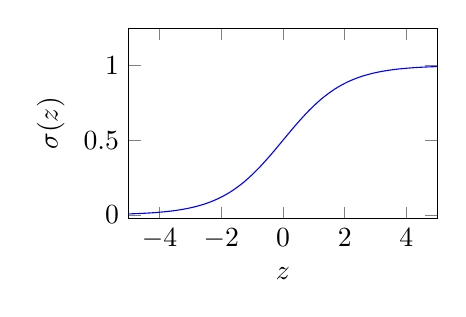
\begin{tikzpicture}
			\begin{axis}[width=5.5cm,height=4cm,ylabel=$\sigma(z)$,xlabel=$z$,ymin=-.025,ymax=1.25,xmin=-5,xmax=5]
				\addplot[blue,smooth] {1/(1+exp(-x))};
			\end{axis}
		\end{tikzpicture}
	}
	\subfigure[Hyperbolic tangent]{
		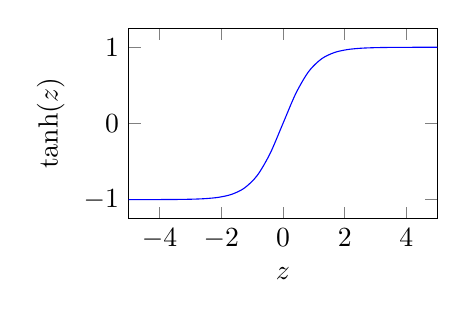
\begin{tikzpicture}
			\begin{axis}[width=5.5cm,height=4cm,ylabel=$\tanh(z)$,xlabel=$z$,ymin=-1.25,ymax=1.25,xmin=-5,xmax=5]
				\addplot[blue,smooth] {tanh(x)};
			\end{axis}
		\end{tikzpicture}
	}
    \subfigure[ReLU]{
		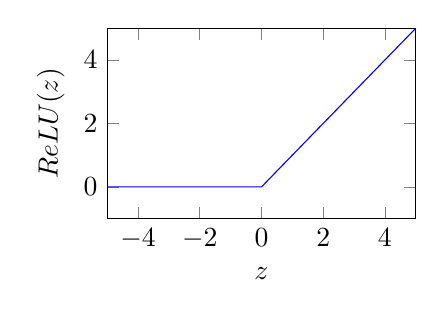
\begin{tikzpicture}
			\begin{axis}[width=5.5cm,height=4cm,ylabel=$ReLU(z)$,xlabel=$z$,ymin=-1,ymax=5,xmin=-5,xmax=5]
				\addplot[blue] {max(0,x)};
			\end{axis}
		\end{tikzpicture}
	}
    \subfigure[Leaky ReLU]{
		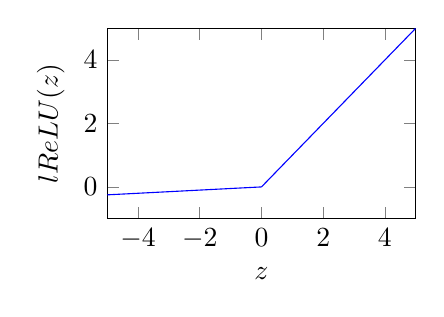
\begin{tikzpicture}
			\begin{axis}[width=5.5cm,height=4cm,ylabel=$lReLU(z)$,xlabel=$z$,ymin=-1,ymax=5,xmin=-5,xmax=5]
				\addplot[blue] {max(0.05*x,x)};
			\end{axis}
		\end{tikzpicture}
	}
    	\caption[Sigmoidal activation functions.]{Commonly used activation functions including the logistic sigmoid $\sigma(z)$, the hyperbolic tangent $tanh(z)$, ReLU and leaky ReLU.}
    	\label{fig:sigmoid-tanh}
\end{figure}
\textbf{Multi-layered Perceptron}
Perceptrons on their own are not powerful enough to generalise to more complex probability distributions. A multilayer perceptron is a collection of fully connected perceptrons, consisting of at least three layers of non-linear activations. Every perceptron is connected with each in the layer in front with a weight $w_{i,j}$. Learning occurs in the perceptron by changing connection weights after each training data is processed, based on the amount of error in the output compared to the expected result, through backpropogation. 

\begin{figure}[H]
	\centering
	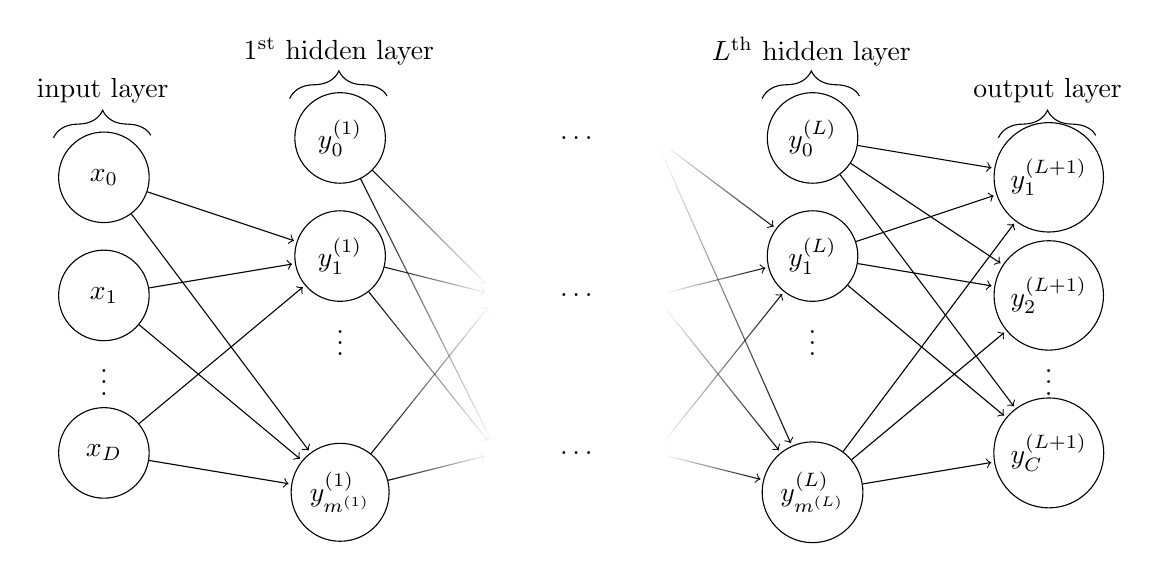
\begin{tikzpicture}[shorten >=1pt]
		\tikzstyle{unit}=[draw,shape=circle,minimum size=1.15cm]
		%\tikzstyle{hidden}=[draw,shape=circle,fill=black!25,minimum size=1.15cm]
		\tikzstyle{hidden}=[draw,shape=circle,minimum size=1.15cm]

		\node[unit](x0) at (0,3.5){$x_0$};
		\node[unit](x1) at (0,2){$x_1$};
		\node at (0,1){\vdots};
		\node[unit](xd) at (0,0){$x_D$};

		\node[hidden](h10) at (3,4){$y_0^{(1)}$};
		\node[hidden](h11) at (3,2.5){$y_1^{(1)}$};
		\node at (3,1.5){\vdots};
		\node[hidden](h1m) at (3,-0.5){$y_{m^{(1)}}^{(1)}$};

		\node(h22) at (5,0){};
		\node(h21) at (5,2){};
		\node(h20) at (5,4){};
		
		\node(d3) at (6,0){$\ldots$};
		\node(d2) at (6,2){$\ldots$};
		\node(d1) at (6,4){$\ldots$};

		\node(hL12) at (7,0){};
		\node(hL11) at (7,2){};
		\node(hL10) at (7,4){};
		
		\node[hidden](hL0) at (9,4){$y_0^{(L)}$};
		\node[hidden](hL1) at (9,2.5){$y_1^{(L)}$};
		\node at (9,1.5){\vdots};
		\node[hidden](hLm) at (9,-0.5){$y_{m^{(L)}}^{(L)}$};

		\node[unit](y1) at (12,3.5){$y_1^{(L+1)}$};
		\node[unit](y2) at (12,2){$y_2^{(L+1)}$};
		\node at (12,1){\vdots};	
		\node[unit](yc) at (12,0){$y_C^{(L+1)}$};

		\draw[->] (x0) -- (h11);
		\draw[->] (x0) -- (h1m);

		\draw[->] (x1) -- (h11);
		\draw[->] (x1) -- (h1m);

		\draw[->] (xd) -- (h11);
		\draw[->] (xd) -- (h1m);

		\draw[->] (hL0) -- (y1);
		\draw[->] (hL0) -- (yc);
		\draw[->] (hL0) -- (y2);

		\draw[->] (hL1) -- (y1);
		\draw[->] (hL1) -- (yc);
		\draw[->] (hL1) -- (y2);

		\draw[->] (hLm) -- (y1);
		\draw[->] (hLm) -- (y2);
		\draw[->] (hLm) -- (yc);
		\draw[->,path fading=east] (h10) -- (h21);
		\draw[->,path fading=east] (h10) -- (h22);
		
		\draw[->,path fading=east] (h11) -- (h21);
		\draw[->,path fading=east] (h11) -- (h22);
		
		\draw[->,path fading=east] (h1m) -- (h21);
		\draw[->,path fading=east] (h1m) -- (h22);
		
		\draw[->,path fading=west] (hL10) -- (hL1);
		\draw[->,path fading=west] (hL11) -- (hL1);
		\draw[->,path fading=west] (hL12) -- (hL1);
		
		\draw[->,path fading=west] (hL10) -- (hLm);
		\draw[->,path fading=west] (hL11) -- (hLm);
		\draw[->,path fading=west] (hL12) -- (hLm);
		
		\draw [decorate,decoration={brace,amplitude=10pt},xshift=-4pt,yshift=0pt] (-0.5,4) -- (0.75,4) node [black,midway,yshift=+0.6cm]{input layer};
		\draw [decorate,decoration={brace,amplitude=10pt},xshift=-4pt,yshift=0pt] (2.5,4.5) -- (3.75,4.5) node [black,midway,yshift=+0.6cm]{$1^{\text{st}}$ hidden layer};
		\draw [decorate,decoration={brace,amplitude=10pt},xshift=-4pt,yshift=0pt] (8.5,4.5) -- (9.75,4.5) node [black,midway,yshift=+0.6cm]{$L^{\text{th}}$ hidden layer};
		\draw [decorate,decoration={brace,amplitude=10pt},xshift=-4pt,yshift=0pt] (11.5,4) -- (12.75,4) node [black,midway,yshift=+0.6cm]{output layer};
	\end{tikzpicture}
	\caption[Network graph for a $(L+1)$-layer perceptron.]{Network graph of a $(L+1)$-layer perceptron with $D$ input units and $C$ output units. The $l^{\text{th}}$ hidden layer contains $m^{(l)}$ hidden units.}
	\label{fig:multilayer-perceptron}
\end{figure}
    
    
\section{Convolution Neural Networks}
Convolution Neural Networks consist of input, hidden and output layers. The hidden layers unlike normal deep neural networks contain convolutional, pooling, fully connected and normalization layers. 

\textbf{Convolutional}\\
The convolutional layer applies a convolution operator to the incoming neuron layer and 

\textbf{Pooling}\\
Pooling layers are used to reduce the size of the layers. They can take multiple neurons from one layer and output a single reduced neuron. For example max pooling is where the maximum value of the cluster of neurons is used as the output, or average pooling where the mean average of the neuron cluster is used. 

\textbf{Fully Connected}\\
A fully connected layer connects every neuron from the input layer to every neuron in the output layer. 

\subsection{Naive Bayes Classifier}

Naive Bayes classifier is a simple probabilistic classifier based on applying Bayes' theorem with naive independence assumptions between the features. This is the major problem with this approach since the features derived from the graphs are likely  dependent on each other, although an advantage of naive Bayes is that it only requires a small number of training data to estimate the parameters necessary for classification.
The Bayes theorem states describes the likelihood of an event A given an event B is true probability, based on prior knowledge of conditions that might be related to the event. 
$$ P(C_k \mid \mathbf{x}) = \frac{P(\mathbf{x} \mid C_k) \, P(C_k)}{P(\mathbf{x})} $$
In reality only the numerator is of interest since the denominator does not depend on the class $\mathbf{C}$ so it is effectively a constant and can be taken out and rewritten as: 
\begin{equation}
\begin{split}
{P(C_k, x_1, x_2, ..., x_n)} & = P(x_1 \mid C_k, x_2, ..., x_n)P(x_2, ... , x_n, C_k) \\
							  & = P(x_1 \mid C_k, x_2, ..., x_n)P(x_2 \mid x_3, ... , x_n, C_k)P(x_3, ... , x_n, C_k) \\
                              & = ...\\
                              & = P(x_1 \mid C_k, x_2, ..., x_n)...P(x_n-1 \mid x_n, C_k)P(x_n \mid x_n, C_k)P(C_k)
\end{split}
\end{equation}
Now with the naive assumption that each feature ${x_i}$ is conditionally independent of one another so:
\begin{equation}
\begin{split}
P(x_i \mid x_i+1, ..., x_n, C_k) = P(x_i \mid C_k)
\end{split}
\end{equation}
Therefore the conditional probability of the class variable C is:
\begin{equation}
\begin{split}
{P(C_k, x_1, x_2, ..., x_n)} & \propto P(C_k){\displaystyle \prod_{i=1}^{n} P(x_i \mid C_k)}
\end{split}
\end{equation}

Finally to construct the naive Bayes classifier the most probable hypothesis is chosen known as the maximum a posteriori decision rule and the corresponding Bayes classifier is the function that assigns a class label $\hat y = C_k$, for some class $C_k$ as:
\begin{equation}
\begin{split}
\hat y = \argmax_k  P(C_k){\displaystyle \prod_{i=1}^{n} P(x_i \mid C_k)}
\end{split}
\end{equation}

\subsection{Support Vector Machines}
Support Vector Machines a represent the training examples as points in space, mapped so that the examples of the separate categories are divided by a clear gap that is as wide as possible. When new examples are observed they are mapped into that same space and predicted to belong to a category based on which side of the gap they fall. SVMs can efficiently perform a non-linear classification using what is called the kernel trick, implicitly mapping their inputs into high-dimensional feature spaces.


\subsection{Decision trees}
The goal is to create a model that predicts the value of a target variable by learning simple decision rules inferred from the data features. It allows the model to be  visualised so the results can be more easily reasoned about compared to other machine learning algorithms which can seem like a black box between the inputs and outputs.  Although the trees are prone to overfit to data, particularly if the tree is deep. 

A rooted tree is constructed with each branch containing observations about the item of data. The observations are used to traverse down the tree until the conclusion about the data is retrieved at the leaf nodes of the tree. 

\begin{figure}[H]
      \caption{Example of a decision tree where $o_i$ are observations about the data and $C_i$ are classes the datum could belong too once traversing the decision tree from the root observation going left or right depending on the outcome of the observation test.}
      
$$\begin{forest}
for tree={l sep+=.8cm,s sep+=.5cm,shape=rectangle, rounded corners,
    draw, align=center,
    top color=white, bottom color=gray!20}
  [$o_0$
     [$o_1$,for children={font=\bfseries},edge label={node[midway,left]{$\checkmark$}} 
       [$C_0$, edge label={node[midway,left]{$\checkmark$}} ]
       [$C_1$, edge label={node[midway,right]{$\times$}}]     
     ]
     [$o_2$,font=\bfseries,edge label={node[midway,right]{$\times$}} 
       [$o_3$,for children={font=\bfseries}, edge label={node[midway,left]{$\checkmark$}}
         [$C_0$, edge label={node[midway,left]{$\checkmark$}} ]
         [$C_1$, edge label={node[midway,right]{$\times$}}]       
       ]
       [$o_4$, for children={font=\bfseries}, edge label={node[midway,right]{$\times$}}
       [$C_1$, edge label={node[midway,left]{$\checkmark$}} ]
       [$C_2$, edge label={node[midway,right]{$\times$}}]]
     ]
]    
\end{forest}
$$
\end{figure}
\subsection{Random Forests}
Random forests are comprised of a multitude of differently constructed decision trees at training time and output the class that is the mode of all the decision tree outputs. Random forests correct the overfitting habit experienced by decision trees\cite{treeoverfit}. They prevent overfitting by constructing many different decision trees using only certain subset of the features vector. Overall, although each tree will only incorporate a small random subset of features, collectively most or all of the features will be utilized by all of the trees. This randomness prevents highly correlated trees since a few features that are particularly predictive could otherwise be used to construct most of the trees with a small training error but so the model would be overfit to this.

\section{Graph Theory}

To use graphs constructed from the user location data as inputs into the traditional supervised machine learning algorithms, the features belonging to the graphs must be extracted from the graphs constructed. I will explain some of the graph features we can extract out to distinguish between graphs that were used in supervised approaches.

\begin{description}
\item [Number of nodes:] the number of nodes in the graph
\item [Number of edges:] the number of edges in the graph
\item [Max degree:] the maximum number of neighbours any node in the graph has
\item [Density:]  Density is defined as: $$\frac{|E|}{|V|(|V| - 1)}$$ for directed graphs, a dense graph is a graph in which the number of edges is close to the maximal number of edges. 
\item [Eccentricity:] Eccentricity of a node is the maximum distance to any other node in the graph. This is a vector as it is defined for each node in the graph and so the mean and variance of the Eccentricity are used as scalar value.
\item [Diameter:] The greatest distance between any two nodes in the graph also the largest eccentricity in the graph.
\item [Radius:] The minimum of the greatest distance between any nodes in the graph also the smallest eccentricity value from any node in the graph.
\item [Centre Size:] The size of the centre of a graph. The centre of a graph is the set of all nodes in the graph which have minimum eccentricity or are the radius of the graph. 
\item [Average Shortest Path Length:] The mean average of the shortest path between all pairs of nodes in the graph. 
\item [Clustering Coefficient:] measure of the degree to which nodes in a graph tend to cluster together. 
\item [Betweenness Centrality:]  The betweenness centrality for each vertex is the number of  shortest paths that pass through the vertex. The shortest path between the vertices's is one where the sum of the weights of the edges is minimized.
\item [Shortest Path Length:] Average and variance of the shortest path lengths in the graph.
\item [Edge Betweenness Centrality:] Vector containing the fraction of shortest paths each edge belongs to. The mean and variance of these are extracted as features.
\item [PageRank:] Computes a ranking of the nodes in the graph based on the structure of the incoming links. 



\end{description}

\section{Software Engineering}
This section deals with the requirements set out, early decisions made and tools and software engineering techniques used to finish and deliver the project in an organised, timely fashion.

\subsection{Requirements}

\subsection{Tools and Libraries}

\textbf{Version Control}\\
I used Git for version control for the project, which was put on my GitHub repository. 
\textbf{Build Tools}\\
I used PyCharm for building and testing the Python code since it contains a great SSH server interface for accessing the dataset stored on its private server and for creating and running Python scripts on that server via my local machine, abstracting away complexities in accessing the private, sensitive information to prevent any leaks of data out of its private server. \\
\textbf{Languages}\\


\subsection{Starting Point}









\chapter{Implementation}
\chapter{Evaluation}
\chapter{Conclusion}

%%%%%%%%%%%%%%%%%%%%%%%%%%%%%%%%%%%%%%%%%%%%%%%%%%%%%%%%%%%%%%%%%%%%%%%%%%%%%%%%
%% Bibliography:
%%
\addcontentsline{toc}{chapter}{Bibliography}
\bibliographystyle{abbrv}
% \bibliography{thesis}
\begin{thebibliography}{99}
\bibitem{approximator} Cybenko, G.V.
Approximation by Superpositions of a Sigmoidal function. In van Schuppen, Jan H. Mathematics of Control, Signals, and Systems. Springer International. pp. 303–314. 2006
\bibitem{Hastie, Trevor; Tibshirani, Robert; Friedman, Jerome (2008). The Elements of Statistical Learning (2nd ed.). Springer. ISBN 0-387-95284-5.}
\end{thebibliography}
%% Appendix:
%%

\appendix

%% Index:
%%
\printthesisindex

\end{document}